\documentclass{beamer}
%\usetheme{PaloAlto}
%\usetheme{Berlin}
\usetheme{Ilmenau}
\usecolortheme{seahorse}

%\usepackage[utf8]{inputenc}
%\usepackage{default}
%\usepackage[italian]{babel}

%\usepackage{titleref}
%\usepackage{zref-titleref}

\usepackage{amsmath}
\usepackage{amssymb}
\usepackage{amsthm}
\usepackage{xfrac}
\usepackage[all]{xy}
\usepackage{mathtools}
\usepackage{graphicx}
%\usepackage{fullpage}
\usepackage{hyperref}
\usepackage[utf8x]{inputenc}
\usepackage[italian]{babel}
\usepackage{mathtools}

%\usepackage{pdftricks}
%\begin{psinputs}
%   \usepackage[pdf]{pstricks}
 %  \usepackage{multido}
%\end{psinputs}

\usepackage{ulem}

\setlength{\parindent}{0in}

\newcounter{counter1}

\theoremstyle{plain}
\newtheorem{myteo}[counter1]{Teorema}
\newtheorem{mylem}[counter1]{Lemma}
\newtheorem{mypro}[counter1]{Proposizione}
\newtheorem{mycor}[counter1]{Corollario}
\newtheorem*{myteo*}{Teorema}
\newtheorem*{mylem*}{Lemma}
\newtheorem*{mypro*}{Proposizione}
\newtheorem*{mycor*}{Corollario}

\theoremstyle{definition}
\newtheorem{mydef}[counter1]{Definizione}
\newtheorem{myes}[counter1]{Esempio}
\newtheorem{myex}[counter1]{Esercizio}
\newtheorem*{mydef*}{Definizione}
\newtheorem*{myes*}{Esempio}
\newtheorem*{myex*}{Esercizio}

\theoremstyle{remark}
\newtheorem{mynot}[counter1]{Nota}
\newtheorem{myoss}[counter1]{Osservazione}
\newtheorem*{mynot*}{Nota}
\newtheorem*{myoss*}{Osservazione}

\newcommand{\obar}[1]{\overline{#1}}
\newcommand{\ubar}[1]{\underline{#1}}

\newcommand{\set}[1]{\left\{#1\right\}}
\newcommand{\pa}[1]{\left(#1\right)}
\newcommand{\ang}[1]{\left<#1\right>}
\newcommand{\bra}[1]{\left[#1\right]}
\newcommand{\abs}[1]{\left|#1\right|}
\newcommand{\norm}[1]{\left\|#1\right\|}

\newcommand{\pfrac}[2]{\pa{\frac{#1}{#2}}}
\newcommand{\bfrac}[2]{\bra{\frac{#1}{#2}}}
\newcommand{\psfrac}[2]{\pa{\sfrac{#1}{#2}}}
\newcommand{\bsfrac}[2]{\bra{\sfrac{#1}{#2}}}

\newcommand{\der}[2]{\frac{\partial #1}{\partial #2}}
\newcommand{\pder}[2]{\pfrac{\partial #1}{\partial #2}}
\newcommand{\sder}[2]{\sfrac{\partial #1}{\partial #2}}
\newcommand{\psder}[2]{\psfrac{\partial #1}{\partial #2}}

\newcommand{\intl}{\int \limits}

\DeclareMathOperator{\de}{d}
\DeclareMathOperator{\id}{Id}
\DeclareMathOperator{\len}{len}

\DeclareMathOperator{\gl}{GL}
\DeclareMathOperator{\aff}{Aff}
\DeclareMathOperator{\isom}{Isom}

\DeclareMathOperator{\im}{Im}



\begin{document}


\title[Un nuovo metodo di regolarizzazione di Tikhonov]{Un nuovo metodo di regolarizzazione di Tikhonov}
\subtitle{Scelta di una nuova matrice di penalizzazione nel caso in
  cui non ne sia nota una dal problema}
\author{Enrico Polesel}
%\institute[Scuola Normale Superiore]{Scuola Normale Superiore}
\date{28 ottobre 2014}

%\author[Enrico Polesel]{\begin{tabular}{r@{ }l}
%Autore: &  Enrico Polesel \\ 
%Relatore: & Andrea Mennucci
%\end{tabular}
%}



\begin{frame}[plain]
  \titlepage
\end{frame}

\begin{frame}[plain]
 \frametitle{Indice}
 \tableofcontents
\end{frame}


%\AtBeginSection[]
%{
%  \begin{frame}{\secname}
%    \tableofcontents[currentsection]
%  \end{frame}
%}


\AtBeginSubsection[]
{
  \begin{frame}[plain]{\secname $\rightarrow$ \subsecname}
    \tableofcontents[currentsubsection]
  \end{frame}
}

\section{Introduzione}

\subsection{Equazioni integrali di Fredholm}

\begin{frame}{L'equazione}
  Molti problemi possono essere modellati con l'equazione
  \begin{block}{Equazione integrale di Fredholm}
    \[ g(t) = \intl _{\Omega} k(t,s) f(s) \de s \]
  \end{block}
  dove $f(s)\in L^2(\Omega)$ è la funzione cercata, $g(s)\in
  L^2(\Omega)$ e la misura che possiamo effettuare e $k(t,s)\in
  L^2(\Omega \times \Omega)$ è detto \textit{kernel}
  \vfill
  
  In modo naturale abbiamo un operatore lineare
  \[ \begin{matrix}
    K:\; &L^2(\Omega) &\longrightarrow &L^2(\Omega)\\
    & f &\longrightarrow & \intl _\Omega k(\cdot , s) f(s) \de s 
  \end{matrix} \]

\end{frame}

\begin{frame}{Componenti ad alta frequenza}
  Per Riemann-Lebesgue abbiamo ( con $\Omega = \mathbb{R}$) che
  l'operatore $K$ attuisce le componenti ad alta frequenza di $f$,
  infatti
  \[ \lim _{z \to \infty} \intl _\mathbb{R} k(t,s) e^{-zs} \de s =
  0 \]

  Quindi da un eventuale $K^{-1}$ ci aspettiamo che questo amplifichi
  l'immagini di tali componenti.
\end{frame}

\begin{frame}{Espansione in valori singolari}
  Sotto opportune ipotesi possiamo scrivere la sua azione come
  \begin{block}{SVE}
    \[ K(v_j) = \sigma _j u_j \]
  \end{block}
  Dove
  \begin{itemize}
  \item $\set{v_i}_{i\in \mathbb{N}}$ è una base ortonormale di
    $L^2(\Omega)$
  \item $\set{u_i}_{i\in \mathbb{N}}$ è una base ortonormale di
    $\im(K)$
  \item $\set{\sigma _i}_{i\in \mathbb{N}}$ sono nonnegativi, $\sigma
    _i \ge \sigma _{i+1}$ e $\sigma _i \to 0$ per $i \to \infty$
  \end{itemize}
\end{frame}

\begin{frame}{Inversa di $K$}
  Per $g \in \im{K}$ possiamo scrivere
  \[ K^{-1}(g) = \sum _{i\in \mathbb{N}} v_i \frac{1}{\sigma _i}
  \ang{g,u_i} \]
  \vfill
  Si può dimostare che $g\in \im (K)$ se e solo se $g$ rispetta le
  condizioni di Picard
  \[ \sum _{i\in \mathbb{N}} \pa{ \frac{1}{\sigma _i} \ang{g,u_i}} ^2
  < \infty \]
\end{frame}

\begin{frame}{Perturbazioni di $g$}
  Osserviamo che una piccola perturbazione di $g$ (dovuta, per
  esempio, all'errore di misura) può non rispettare le condizioni di
  Picard:
  \begin{align*}
    & \sum _{i\in \mathbb{N}} \pa{ \frac{1}{\sigma _i} \ang{\tilde
        g,u_i}} ^2 = \sum _{i\in \mathbb{N}} \pa{ \frac{1}{\sigma _i}
      \ang{g + \varepsilon,u_i}} ^2 = \\
    = & \sum _{i\in \mathbb{N}} \pa{ \frac{1}{\sigma _i}        
      \pa{ \ang{g, u_i} + \ang{ \varepsilon, u_i } } }
%    = \\
%    =&\underbrace{\sum _{i\in \mathbb{N}} \pa{
%          \frac{1}{\sigma _i} \ang{g,u_i}} ^2} _{<\infty}
%    + \underbrace{\sum _{i\in \mathbb{N}} \pa{ \frac{1}{\sigma _i}
%      \ang{\varepsilon,u_i}} ^2} _{???}
  \end{align*}
\end{frame}

\begin{frame}{Discretizzazione}
  Per risolvere numericamente un'equazione integrale di Fredholm
  dobbiamo discretizzare il problema, possiamo decidere di farlo
  prima o dopo la regolarizzazione.
  \vfill
  
  Metodi comuni di discretizzazione sono metodi di collocazione e
  metodi di proiezione.
  \vfill
  
  Se discretizziamo il problema prima di regolarizzarlo allora
  otterremo una matrice mal condizionata.
\end{frame}



\subsection{Sistemi lineari mal condizionati}

\begin{frame}{Esempi}
  Abbiamo già osservato che se discretizziamo un'equazione integrale di
  Fredholm senza regolarizzarla otteniamo una matrice mal
  condizionata.
  \vfill
  
  Nel cercare gli zeri di alcune funzioni con il metodo di Newton
  capita che lo Jacobiano risultante sia mal condizionato, questo è un
  altro caso in cui è necessaria una regolarizzazione.
\end{frame}

\begin{frame}{Il problema}
  Sia $A\in \mathbb{R}^{m \times n}$ una matrice con $m \ge n$ e $b
  \in \mathbb{R}^m$, il nostro problema è trovare $x \in \mathbb{R}^n$
  tale che $Ax = b$, visto che il problema potrebbe essere impossibile
  allora chiediamo di trovare
  \[ x = \arg\min _{x\in \mathbb{R}^n} \pa{ \norm{Ax -b} } \]
  per una qualche norma $\norm{\cdot}$. Noi useremo $\norm{\cdot}_2$.
\end{frame}

\begin{frame}{Decomposizione in valori singolari}
  Sappiamo che possiamo scrivere
  \begin{block}{SVD}
    \[ A = U\Sigma V^T \] 
  \end{block}
  con $V\in \mathbb{R}^{n\times n}$,$U\in \mathbb{R}^{m\times m}$
  ortogonali, $\set{\sigma _i}_{i=1..n}$ nonnegativi con $\sigma _i
  \ge \sigma _{i+1}$ e tali che
%  \[ \Sigma = \begin{pmatrix}
%    \sigma _1 & & & \\
%    & \sigma _2 & &  \\
%    & & \ddots & \\
%    & & & \sigma _n 
%  \end{pmatrix} \]
  \[ \Sigma = \mathrm{diag} \pa{ \sigma_1,...,\sigma _n} \]
  
  Possiamo anche scrivere
  \[ Ax = \sum _{i=1} ^n u_i \sigma _i \ang{v_i,x} \]
\end{frame}

\begin{frame}{Pseudoinversa di Moore-Penrose}
  Dalla scomposizione in valori singolari di $A$ possiamo scrivere la
  soluzione del nostro problema di minimizzazione
  \[ x = \sum _{i=1} ^k \frac{1}{\sigma _i} v_i \ang{u_i,b} \]
  \[ x = A^+ b \]
  \begin{block}{Pseudoinversa di Moore-Penrose}
    \[ A^+ = \sum _{i=1} ^k \frac{1}{\sigma _i} v_i u_i ^T\]
  \end{block}
  dove $k$ è il rango di $A$
%  \[ k = \max \set{ i :\; \sigma_i \neq 0 } \]
\end{frame}

\begin{frame}{Condizionamento}
  Sappiamo che il condizionamento di $A$ si può scrivere come
  \begin{block}{Condizionamento in funzione dei valori singolari}
    \[ \kappa (A) = \norm{A^+}_2\norm{A}_2 = \frac{\sigma _1}{\sigma
    _k} \]
  \end{block}

  Quindi per matrici mal condizonate avremo che $\sigma _k$ sarà
  piccolo (rispetto a $\sigma_1$)
\end{frame}

\begin{frame}{Effetto di errori in $b$}
  Supponendo che $\tilde b = b+ \varepsilon$, cioè è affetto da
  errore, abbiamo che 
  
  \begin{align*}
    x =& \sum _{i=1} ^k \frac{1}{\sigma _i} v_i \ang{u_i,b +
      \varepsilon} = \\
    =& \sum _{i=1} ^k \frac{1}{\sigma _i} v_i \ang{u_i,b} + \sum
    _{i=1} ^k \frac{1}{\sigma _i} v_i \ang{u_i,\varepsilon}
  \end{align*}

  Ed infatti, come ci aspettavamo, piccoli valori di $\sigma_k$
  amplificano di molto l'errore introdotto da $\varepsilon$.
\end{frame}


\section{Metodi di regolarizzazione}

\subsection{Introduzione}

\begin{frame}{Esempio}
  \begin{figure}
    \centering
    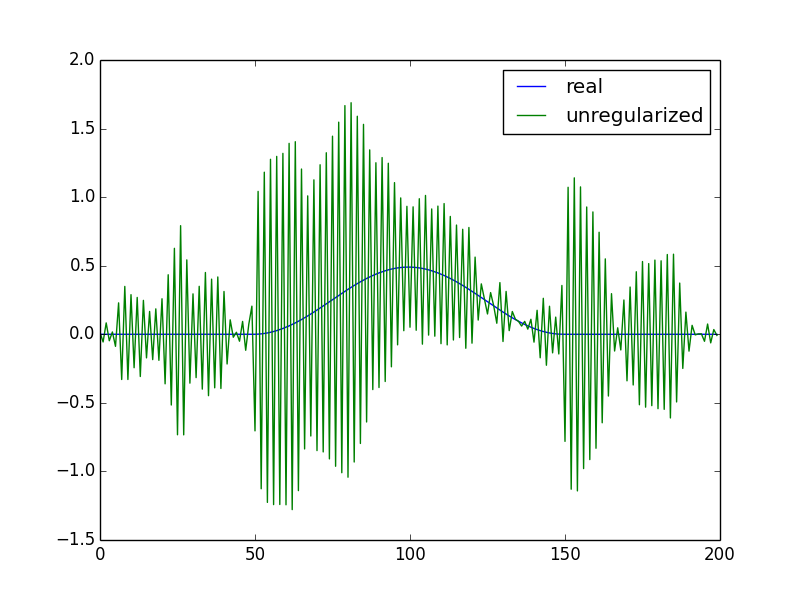
\includegraphics[keepaspectratio,width=190px]{phillips_unreg_-6.png}
    \caption{Problema phillips con un errore relativo di $10^{-6}$ sul
      vettore dei termini noti}
  \end{figure}
\end{frame}


\begin{frame}{Problema}
  Supponiamo di avere $A\in \mathbb{R}^{m \times n}$ mal condizionata
  e $\tilde b = b + \varepsilon$ vettore dei termini noti
  ``rumoroso''. Cerchiamo un $\tilde x$ tale che
  \begin{itemize}
  \item $\norm{A\tilde x-\tilde b}$ sia vicino $\min \limits_x
    \pa{\norm{A x - \tilde b}}$
  \item $\tilde x$ sia stabile per piccole variazioni di $\tilde b$,
    cioè chiediamo che la soluzione sia ``regolare''
  \end{itemize}
\end{frame}

\begin{frame}{Fattori di filtro}
  \begin{mydef}
    Data una matrice $A$ e un metodo di regolarizzazione diciamo che
    quest'ultimo ha fattori di filtro $\pa{\varphi _i}$ se la
    soluzione può essere scritta come
    \[ x = \sum _{i=1} ^k \varphi _i \frac{1}{\sigma _i} v_i
    \ang{u_i,\tilde b} \]
  \end{mydef}

  Osserviamo che se tutti i fattori di filtro sono uguali a $1$ allora
  otteniamo la soluzione non regolarizzata.
\end{frame}

\subsection{TSVD}

\begin{frame}{Il metodo}
  Abbiamo già osservato che
  \[ \kappa (A) = \frac{\sigma _1}{\sigma _k} \]
  
  Un metodo molto semplice di regolarizzazione è annullare i valori
  singolari piccoli, cioè sostituire $A$ con
  \[ A_\alpha = \sum _{i=1} ^\alpha u_i \sigma _i v_i ^T \]
  dove $1\le \alpha \le k$ intero.
  \vfill
  
  Il suo condizionamento sarà
  \[ \kappa (A_\alpha) = \frac{\sigma _1}{\sigma _\alpha} \le
  \frac{\sigma _1}{\sigma _k} = \kappa(A) \]
\end{frame}

\begin{frame}{Fattori di filtro}
  La soluzione del problema regolarizzato con la TSVD di parametro
  $\alpha$ è
  \[ x_\alpha = A_\alpha ^+ \tilde b = \sum _{i=1} ^\alpha
  \frac{1}{\sigma _i} v_i \ang{u_i,\tilde b} \]
  \vfill

  Quindi i fattori di filtro sono
  \begin{block}{Fattori di filtro della TSVD}
  \[ \varphi ^{\text{TSVD}}_{\alpha,i} = \left\{
    \begin{matrix}
      1 \; &1\le i \le \alpha\\
      0 \; &\alpha < i \le k
    \end{matrix}
    \right. \]
  \end{block}
  \vfill
  
  Quindi questo approcio ignora completamente le componenti $u_i,
  i>\alpha$ di $\tilde b$.
\end{frame}

\begin{frame}{Parametro di regolarizzazione}
  La soluzione regolarizzata dipende dalla scelta del parametro
  $\alpha$. Vediamo che:
  \begin{itemize}
  \item per valori troppo grandi di $\alpha$ la matrice $A_\alpha$
    rimane mal condizionata
  \item per valori troppo piccoli di $\alpha$ la matrice $A_\alpha$ è
    troppo diversa da $A$ e il problema non rispetta più il problema
    orginale
  \end{itemize}
\end{frame}


\subsection{Regolarizzazione di Tikhonov}

\begin{frame}{Tikhonov standard}
  Modifichiamo il problema cercando
  \[ x_\mu = \arg\min _{x \in \mathbb{R}^n} \pa{ \norm{Ax -\tilde b}^2
    + \mu\norm{x}^2} \]
  \vfill
  
  In questo modo penalizziamo soluzioni di norma grande derivanti
  dall'amplificazione dell'errore da parte dei valori singolari piccolo
\end{frame}

\begin{frame}{Tikhonov generale}
  In generale possiamo scrivere la regolarizzazione di Tikhonov come
  \begin{block}{Forma generale di Tikhonov}
  \[ x_\mu = \arg\min _{x \in \mathbb{R}^n} \pa{ \norm{Ax -\tilde b}^2 +
    \norm{L_\mu x}^2} \]
  \end{block}
  con $L_\mu$ una matrice di penalizzazione.

  In alcuni casi è utile usare questa forma perché è nota (dal
  problema) una buona matrice di penalizzazione $L$ e quindi si prende
  $L_\mu = \mu L$.
  \vfill

  Se $L_\mu = \mu I$ allora ritorniamo alla regolarizzazione di
  Tikhonov standard.
\end{frame}

\begin{frame}{Soluzione}
  Riscriviamo il problema di minimo come
  \[ x_\mu = \arg\min _{x \in \mathbb{R}^n} \pa{ \norm{ 
      \begin{pmatrix}
        A \\
        L_\mu
      \end{pmatrix}
      x_\mu -
      \begin{pmatrix}
        \tilde b\\
        0
      \end{pmatrix}
      }^2 }\]
  la soluzione è data dall'equazione
  \[ \begin{pmatrix}
    A^T & L_\mu ^T
  \end{pmatrix}
  \begin{pmatrix}
    A \\
    L_\mu
  \end{pmatrix}
  x_\mu = 
  \begin{pmatrix}
    A^T & L_\mu ^T
  \end{pmatrix}
  \begin{pmatrix}
    \tilde b\\
    0
  \end{pmatrix} \]
  che può essere riscritta come
  \[ \pa{ A^T A + L_\mu^T L_\mu } x_\mu = A^T \tilde b  \]
\end{frame}

\begin{frame}
  Se supponiamo ora che $L_\mu = \mu I$ e che $A = U\Sigma V^T$
  possiamo scrivere
  \[  x_\mu = \pa{ V \Sigma ^2 V^T + \mu ^2 I }^{-1} V \Sigma U^T \tilde b  \]
  \[  x_\mu = V^T \pa{\Sigma ^2 + \mu ^2 I }^{-1} \Sigma U^T \tilde b \]
  \[  x_\mu = V^T
  \begin{pmatrix}
    \frac{\sigma _1 }{\sigma _1 ^2 + \mu ^2} \\
    & \frac{\sigma _2 }{\sigma _2 ^2 + \mu ^2} \\
    & & \ddots \\
    & & & \frac{\sigma _k }{\sigma _k ^2 + \mu ^2}\\
    & & & & 0\\
    & & & & & \ddots \\
    & & & & & & 0
  \end{pmatrix}
  U^T \tilde  b \]
\end{frame}

\begin{frame}{Fattori di filtro}
  Dalla scrittura della soluzione otteniamo che i fattori di filtro
  per Tikhonov standard sono
  \begin{block}{Fattori di filtro per Tikhonov standard}
  \[ \varphi ^{\text{Tikhonov}} _{\mu,i} = \frac{\sigma _i ^2}{\sigma _i
    ^2 + \mu ^2} \]
  \end{block}
  \vfill
  
  Quindi questo metodo da una parte, a differenza della TSVD, tiene
  conto di tutte le componenti di $\tilde b$, dall'altra le attenua
  tutte, comprese quelle ``regolari''
\end{frame}


\subsection{Una nuova matrice di regolarizzazione}

\begin{frame}{La matrice}
  Un compormesso tra i due metodi sopra esposti si trova utilizzando
  la seguente matrice nella regolarizzazione di Tikhonov:
  \[ L_\mu = D _\mu V^T \]
  con
  \[ D_\mu = \mathrm{diag}\pa{ \sqrt{\max\set{\mu ^2 - \sigma _1
        ^2,0}} , ..., \sqrt{\max\set{\mu ^2 - \sigma _n ^2,0}} } \]
\end{frame}

\begin{frame}{La soluzione}
  Possiamo calcolare la soluzione a questo problema
  \begin{align*}
    x_\mu =& \pa{ A^T A + L_\mu^T L_\mu }^{-1} A^T \tilde b = \\
    = & \pa{ V \Sigma ^2 V^T + V D_\mu ^2 V^T} ^{-1} V\Sigma U^T \tilde
    b = \\
    = & V \pa{ \Sigma ^2 + D_\mu ^2 } ^{-1} \Sigma U^T \tilde b \\
    = & \sum _{i=1} ^k \frac{\sigma _i}{\sigma _i ^2 + \max\set{
      \mu ^2 - \sigma _i ^2 ,0}  }  v_i \ang{u_i,\tilde b}
  \end{align*}
\end{frame}

\begin{frame}{I fattori di filtro}
  \begin{block}{Fattori di filtro del nuovo metodo}
    \[ \varphi ^{\text{new}} _{\mu,i} = \frac{\sigma _i ^2}{\sigma _i ^2 + \max\set{
        \mu ^2 - \sigma _i ^2 ,0}  } = \left\{
      \begin{matrix}
        1\; & \sigma _i \ge \mu \\
        \frac{\sigma _i ^2}{\mu ^2} \; & \sigma _i < \mu
      \end{matrix}
    \right. \]
  \end{block}
  \vfill
  
  Quindi, come nella TSVD, non vengono attenuate le componenti con
  $\sigma _i \ge \mu$, mentre le restanti vengono attenuate ma senza
  essere eliminate.
\end{frame}

\begin{frame}{Ottimalità di $L_\mu ^T L_\mu$ in norma}
  Vista la forma della soluzione $x_\mu = \pa{ A^T A + L_\mu^T L_\mu
  }^{-1} A^T \tilde b$ possiamo aspettarci che la differenza tra il
  problema originale sia in un qualche modo misurata da 
  \[ \norm{ \pa{ A^T A + L_\mu^T L_\mu } - A^T A } \]
  
  D'altra parte vogliamo anche che il problema sia regolare, questa
  proprietà si misura con il numero di condizionamento di $\pa{ A^T A
    + L_\mu^T L_\mu }$, per quanto detto precedentemente possiamo
  pensare di usare, per confrontare due matrici, il loro autovalore
  più piccolo (supponendo che i metodi non modifichino di molto
  l'autovalore più grande di $A^T A$).
\end{frame}

\begin{frame}
  Abbiamo il seguente teorema:
  \begin{myteo}
    Sia $M \in \mathbb{R}^{n\times n}$ una matrice simmetrica con
    fattorizzazione spettrale $M = V \Lambda V^T$, dove $V \in
    \mathbb{R}^{n \times n}$ è ortogonale e  $\Lambda = \mathrm{diag} \pa{
      \lambda _1, ... \lambda _n}$. Supponiamo che  $\eta \ge \min _{1\le
      j\le n} \lambda _j$ e sia $C_\eta = \mathrm{diag}
    \pa{ c_1 , ... c_n}\in \mathbb{R}^{n\times n}$ con componenti $c_j
    = \max \set{\eta - \lambda _j, 0}$.
    
    Allora $M + V C_\eta V^T$ ha autovalore più piccolo $\eta$
    e la distanza in norma 2 fra $M$ e la matrice simmetrica più vicina
    con autovalore più piccolo $\eta$ è $\norm{ C_\eta }_2$
  \end{myteo}
  
  Possiamo applicare questo teorema con $M = A^T A$ (e quindi $\lambda
  _j = \sigma _j ^2$), $\eta = \mu ^2$ e $C_\eta = D_\mu ^2$
  e otteniamo che questo metodo è ottimale in norma 2, in particolare
  ritorna una soluzione più accurata del metodo di Tikhonov standard.
\end{frame}

\section{Scelta del parametro di regolarizzazione}

\subsection{Introduzione}

\begin{frame}{Il parametro}
  Tutti i metodi che abbiamo visto dipendono dalla scelta di un
  parametro di regolarizzazione, nei nostri casi questo parametro è un
  intero oppure un reale.
  \vfill

  In altri metodi di regolarizzazione questo parametro potrebbe essere
  anche un vettore, tralasceremo questo caso.
\end{frame}

\begin{frame}{Metodi}
  Sono stati studiati vari metodi per la ricerca del parametro di
  regolarizzazione, per esempio citiamo:
  \begin{itemize}
  \item Il discrepancy principle
  \item Il metodo della L-curve
  \item La General Cross Validation (GCV)
  \end{itemize}
  \vfill
  
  Noi vedremo solo il primo.
\end{frame}

\subsection{Il discrepancy principle}

\begin{frame}{Definizione}
  Supponiamo di avere una buona approssimazione dell'errore di misura
  $\norm{\varepsilon} = \norm{\tilde b - b}$, allora prendiamo la
  soluzione più regolare che non superi tale soglia di errore, cioè
  come parametro di regolarizzazione prendiamo:
  \[ \lambda _\varepsilon = \max \set { \lambda :\; \norm{ Ax_\lambda -
      \tilde b} \le \eta \norm{\varepsilon}} \]
  (dove, per semplicità, abbiamo supposto che la soluzione diventi più
  regolare al crescere di $\lambda$)

  $\eta >1$ è una costante indipendente da $\norm{\varepsilon}$ data
  dall'utente.
\end{frame}

\begin{frame}{Convergenza}
  Si può mostrare che
  \begin{block}{Convergenza nel discrepancy principle}
    \[ \lim \limits _{\norm{\varepsilon} \to 0} x _\varepsilon = x \]
  \end{block}
  Dove $x_\varepsilon = x_{\lambda _ \varepsilon}$ è la soluzione
  ottenuta regolarizzando con il parametro dato dal discrepancy
  principle con $\norm{\varepsilon}$ e $x$ è la soluzione del problema
  non perturbato.
\end{frame}

\begin{frame}{Discrepancy principle e fattori di filtro}
  Se il nostro metodo può essere scritto con i fattori di filtro
  allora possiamo scrivere
  \begin{align*}
    \norm{ Ax_\lambda - \tilde b } =& \norm{ U \Sigma V^T V F \Sigma
      ^{-1} U^T \tilde b - \tilde b} =\\
    =& \norm { U F U^T \tilde b - \tilde b} =\\
    = & \norm{ F U^T \tilde b - U^T \tilde b } =\\
    =& \norm{ \pa{F-I} U^T \tilde b} =\\
    =& \sqrt{\sum _{i=1} ^n \bra{ \pa{ \varphi _i -1} \ang{ u_i, \tilde b} } ^2}
  \end{align*}
\end{frame}

\begin{frame}{Calcolo del parametro di regolarizzazione}
  Per i metodi che abbiamo visto il calcolo del parametro di
  regolarizzazione può essere fatto con:
  \begin{itemize}
  \item per la TSVD abbiamo $\norm{ Ax_\alpha - \tilde b } =
    \sqrt{\sum _{i=\alpha +1} ^n \bra{ \ang{ u_i, \tilde b} } ^2 }$ e
    la soluzione di $\norm{ Ax_\alpha - \tilde b } <\eta
    \norm{\varepsilon}$ si trova esaminando i possibili $n$ valori di
    $\alpha$
  \item Per il metodo di Tikhonov possiamo applicare il metodo di
    Newton alla funzione \[f(\mu) = \sum _{i=1} ^n \bra{ \pa{ \varphi
        _{\mu,i} -1} \ang{ u_i, \tilde b} } ^2 - \eta ^2
    \norm{\varepsilon} ^2 \].
  \end{itemize}
\end{frame}

\section{Esperimenti numerici}

\subsection{Implementazione}

\begin{frame}{Linguaggio}
  I metodi sopra descritti sono stati implementati in Python 2.7.3 con
  l'ausilio della libreria numpy 1.6.2 per i calcoli numerici e pytave
  r51 per poter utilizzare la libreria regtools (scritta da  Per
  Christian Hansen in MATLAB) da cui sono stati ottenuti gli esempi.
  \vfill
  
  L'aritmetica usata è a 64 bit con precisione $2\cdot 10^{-16}$.
\end{frame}

\begin{frame}{Esempi}
  Sono stati usati tre esempi dalla libreria regtools risultati dalla
  discretizzazione di equazioni integrali di Fredholm
  \begin{center}
    \begin{tabular}[c]{c | c}
      \textbf{Problem} & \textbf{Discretization} \\
      \hline
      phillips & Galkerin \\
      shaw & quadrature \\
      ilaplace & quadrature 
    \end{tabular}
  \end{center}
  \vfill
  
  Ogni esempio è stato testato modificando il vettore dei termini noti
  $b$ con un errore relativo del $0.1\%, 1\%, 5\%$ e $10\%$ per poi
  applicare i tre metodi studiati.  
\end{frame}

\subsection{phillips}

\begin{frame}{Risultati}
  Vediamo l'errore relativo $\frac{\norm{\tilde x - x}}{\norm{x}}$
  ottenuto coi vari metodi
  \begin{center}
    \begin{tabular} { c | c | c | c }
err. & TSVD & st. Tik & new Tik \\ \hline 
0.1\% & $0.0138195825427$ & $0.0116105396417$ & $0.00983516140485$ \\
1.0\% & $0.0260978547974$ & $0.0285233863711$ & $0.0267510907107$ \\
5.0\% & $0.0318297867094$ & $0.0599294125318$ & $0.0497013382702$ \\
10.0\% & $0.112628270812$ & $0.10340205612$ & $0.0768979135972$ \\
\end{tabular}

  \end{center}
\end{frame}

\begin{frame}
  \begin{figure}
    \centering
    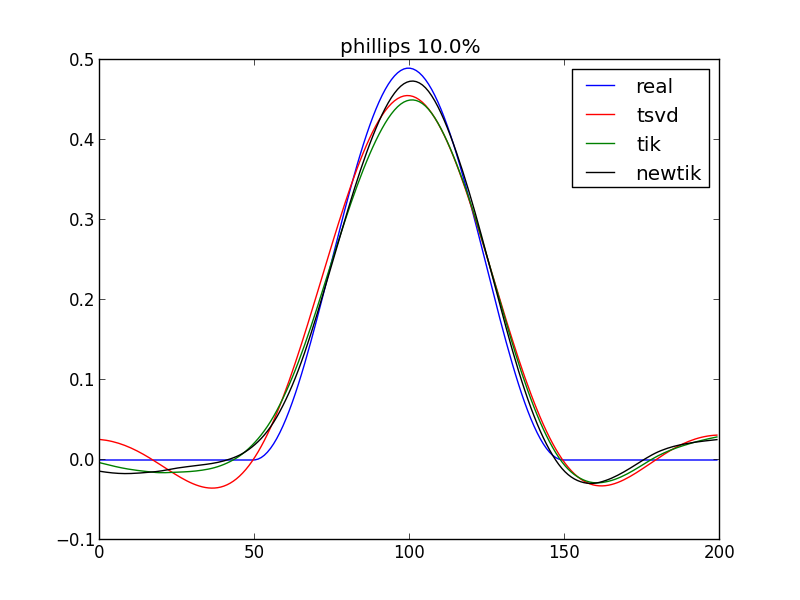
\includegraphics[keepaspectratio,width=270px]{phillips_100.png}
  \end{figure}
\end{frame}

\begin{frame}
  \begin{figure}
    \centering
    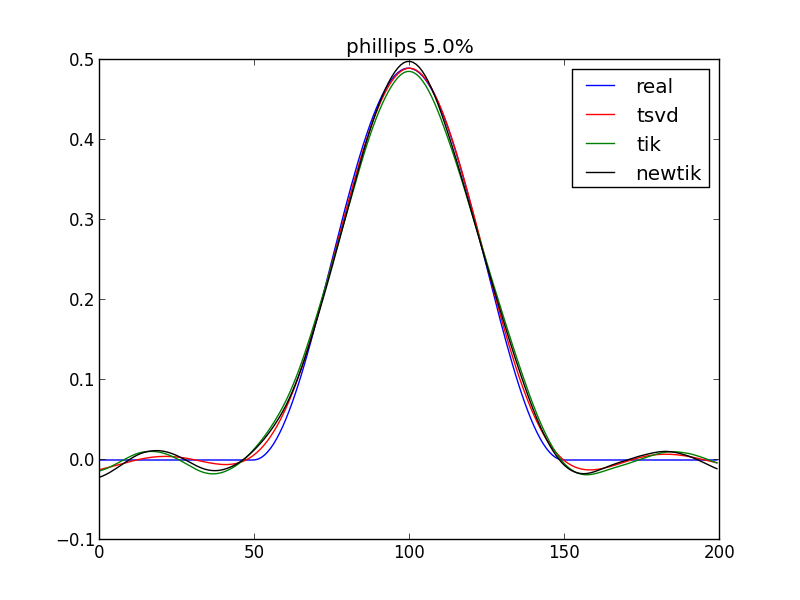
\includegraphics[keepaspectratio,width=270px]{phillips_50.png}
  \end{figure}
\end{frame}

\begin{frame}
  \begin{figure}
    \centering
    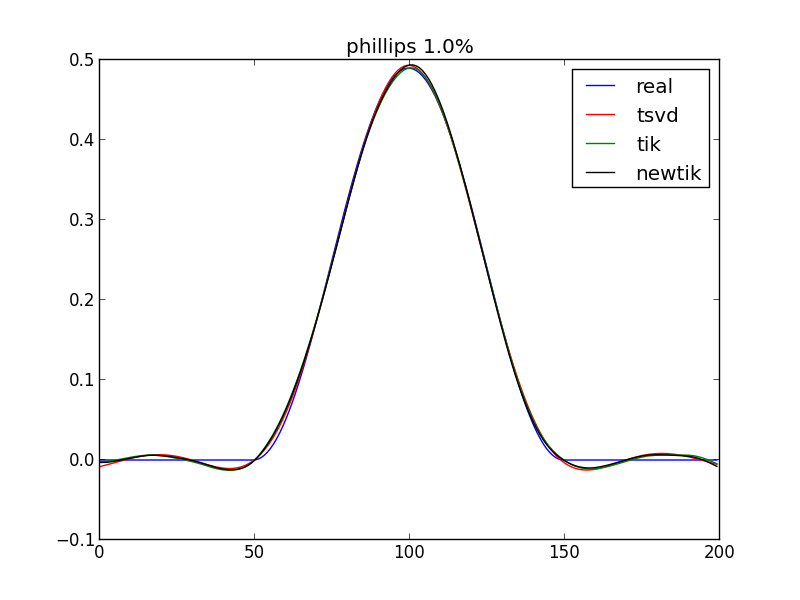
\includegraphics[keepaspectratio,width=270px]{phillips_10.png}
  \end{figure}
\end{frame}

\begin{frame}
  \begin{figure}
    \centering
    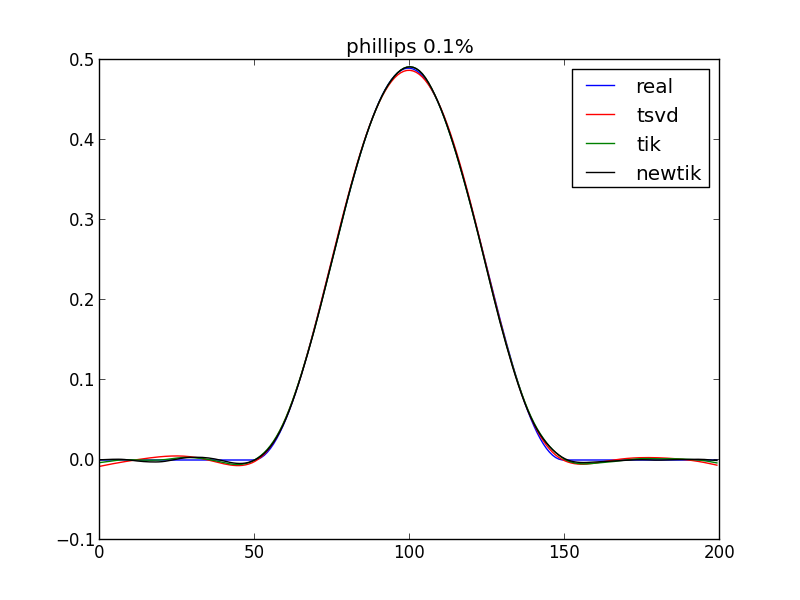
\includegraphics[keepaspectratio,width=270px]{phillips_1.png}
  \end{figure}
\end{frame}


\subsection{shaw}

\begin{frame}{Risultati}
  Vediamo l'errore relativo $\frac{\norm{\tilde x - x}}{\norm{x}}$
  ottenuto coi vari metodi
  \begin{center}
    \begin{tabular} { c | c | c | c }
err. & TSVD & st. Tik & new Tik \\ \hline 
0.1\% & $0.0484473096707$ & $0.0521364537753$ & $0.0538767935587$ \\
1.0\% & $0.0693947164532$ & $0.0640383355947$ & $0.0665150963178$ \\
5.0\% & $0.170684971422$ & $0.156523338342$ & $0.153967028942$ \\
10.0\% & $0.17261152037$ & $0.171708785138$ & $0.163548725702$ \\
\end{tabular}

  \end{center}
\end{frame}

\begin{frame}
  \begin{figure}
    \centering
    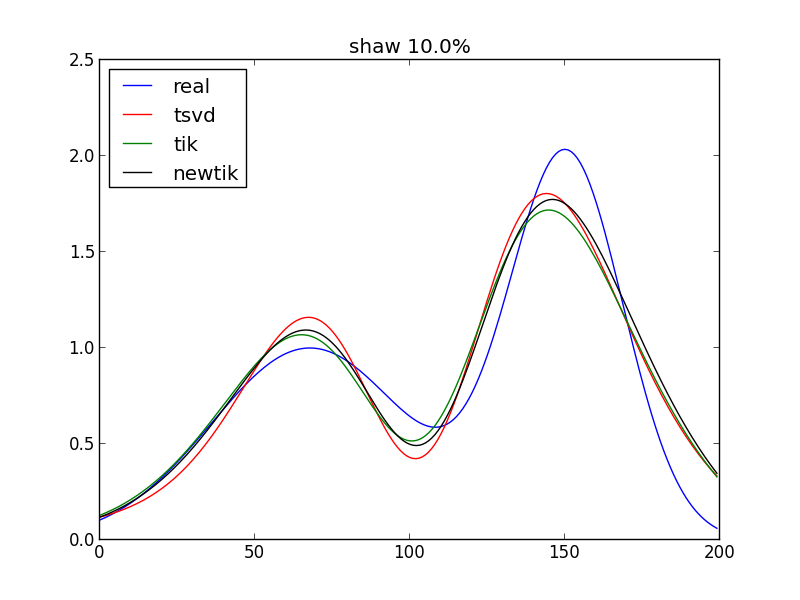
\includegraphics[keepaspectratio,width=270px]{shaw_100.png}
  \end{figure}
\end{frame}

\begin{frame}
  \begin{figure}
    \centering
    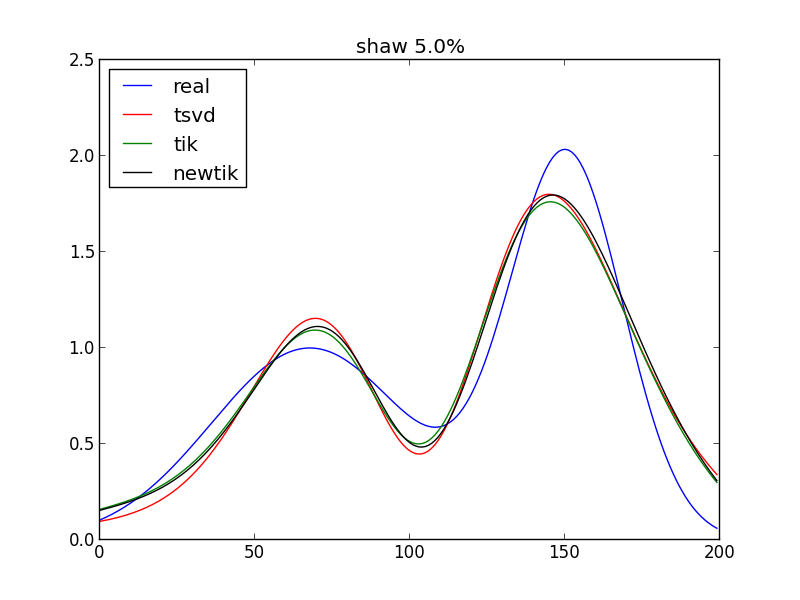
\includegraphics[keepaspectratio,width=270px]{shaw_50.png}
  \end{figure}
\end{frame}

\begin{frame}
  \begin{figure}
    \centering
    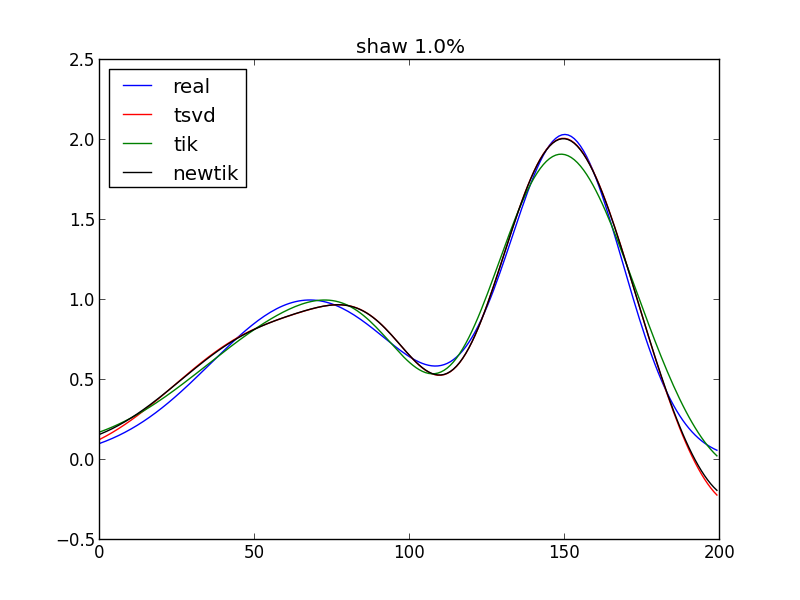
\includegraphics[keepaspectratio,width=270px]{shaw_10.png}
  \end{figure}
\end{frame}

\begin{frame}
  \begin{figure}
    \centering
    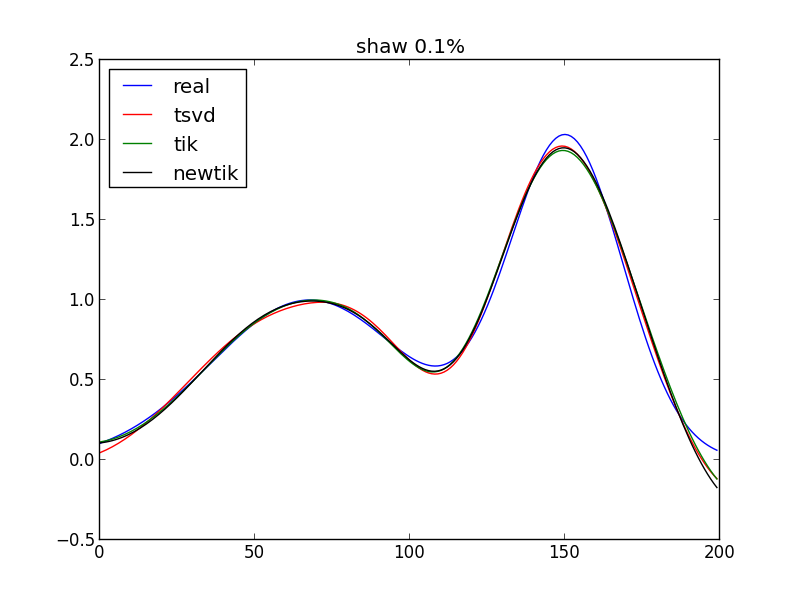
\includegraphics[keepaspectratio,width=270px]{shaw_1.png}
  \end{figure}
\end{frame}


\subsection{ilaplace}

\begin{frame}{Risultati}
  Vediamo l'errore relativo $\frac{\norm{\tilde x - x}}{\norm{x}}$
  ottenuto coi vari metodi
  \begin{center}
    \begin{tabular} { c | c | c | c }
err. & TSVD & st. Tik & new Tik \\ \hline 
0.1\% & $0.157777948817$ & $0.143884144024$ & $0.143913575113$ \\
1.0\% & $0.19650647166$ & $0.187962436226$ & $0.181100803466$ \\
5.0\% & $0.224278999822$ & $0.20894956006$ & $0.202903579018$ \\
10.0\% & $0.229596282931$ & $0.223651132721$ & $0.22435870577$ \\
\end{tabular}

  \end{center}
\end{frame}

\begin{frame}
  \begin{figure}
    \centering
    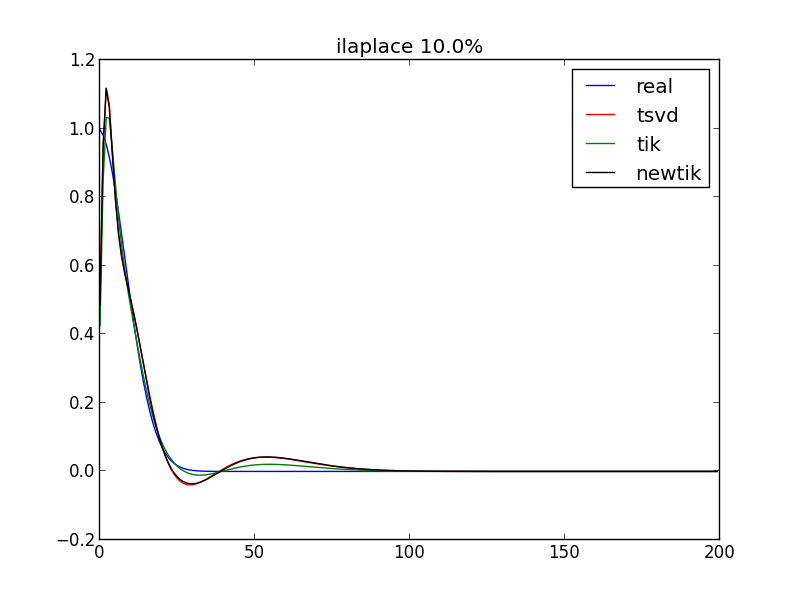
\includegraphics[keepaspectratio,width=270px]{ilaplace_100.png}
  \end{figure}
\end{frame}

\begin{frame}
  \begin{figure}
    \centering
    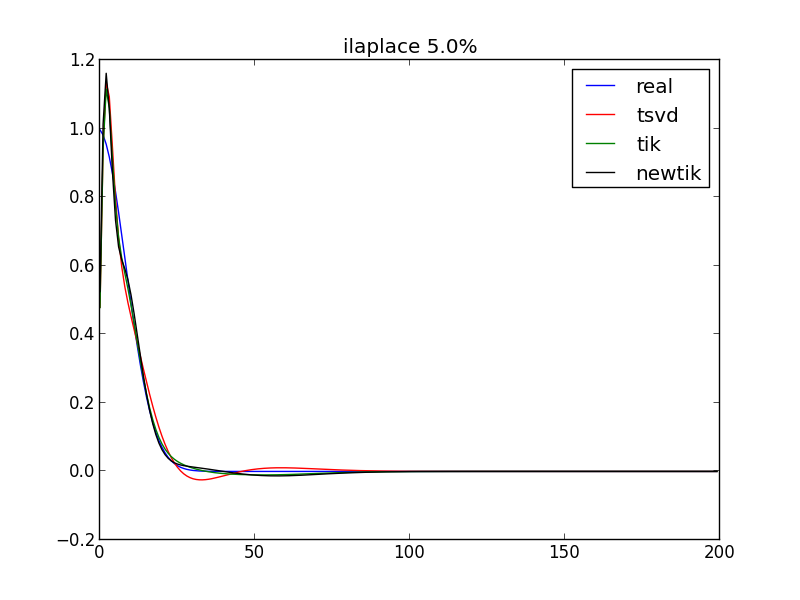
\includegraphics[keepaspectratio,width=270px]{ilaplace_50.png}
  \end{figure}
\end{frame}

\begin{frame}
  \begin{figure}
    \centering
    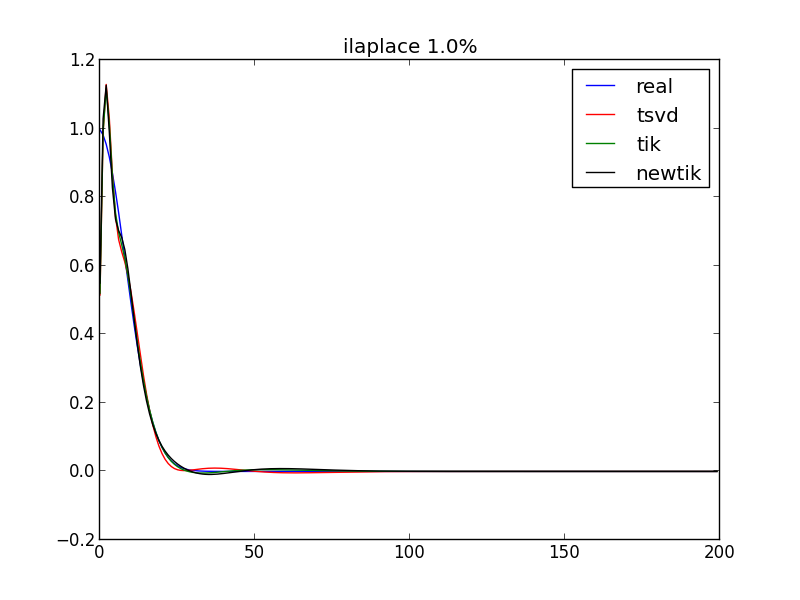
\includegraphics[keepaspectratio,width=270px]{ilaplace_10.png}
  \end{figure}
\end{frame}

\begin{frame}
  \begin{figure}
    \centering
    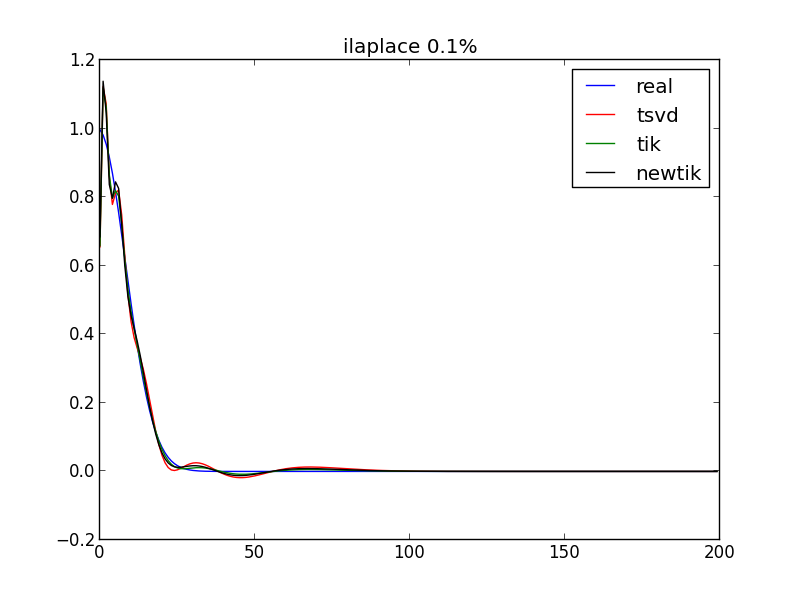
\includegraphics[keepaspectratio,width=270px]{ilaplace_1.png}
  \end{figure}
\end{frame}





\end{document}







